\section{Conceptual models of Experimentation on SE}\label{sec:annex-models-SE}

Las figuras contienen t�rminos en Espa�ol, idioma en que se realiz� la investigaci�n. Hemos preferido no traducir las figuras para asegurar la trazabilidad entre en art�culo y la raw data, disponible en \url{}\odnote{RODRIGO: Indicar ubicaci�n de la raw data}.

\begin{figure*}[htbp!]
	\centering
	\captionsetup{justification=centering}
	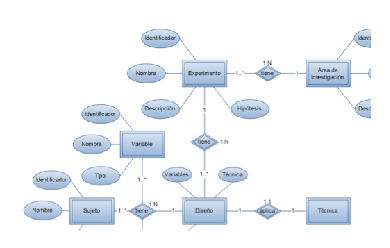
\includegraphics[width=\textwidth]{images/Producto-Intermedio-Revision-Lit}
	\caption{Modelo conceptual preliminar resultado del an�lisis de la literatura relevante.}
	\label{fig-conceptos-preliminar}
	\odnote{RODRIGO: He movido la figura a un anexo. Que se vea entera. D�jala en Espa�ol, ya que es posible que haya que haya que enlazar a ese ap�ndice el resto del row data de la tesis}
\end{figure*}

\begin{figure*}[htbp!]
	\centering
	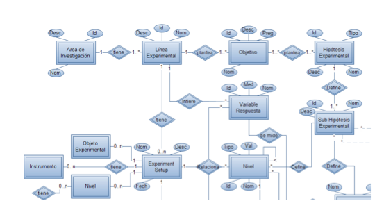
\includegraphics[width=5in]{images/Producto-Final-Revision-Lit}
	\caption{Modelo conceptual resultado del an�lisis de los materiales experimentales.}
	\label{fig-conceptos-final-revision-fuentes}\odnote{RODRIGO: Pon el modelo completo.}
\end{figure*}

\begin{figure*}[htbp!]
	\centering
	\includegraphics[width=5in]{images/Producto-Final-Observacion-Par}
	\caption{Modelo conceptual resultado de la observaci�n participativa.}
	\label{fig-conceptos-final-observacion-participativa}\odnote{RODRIGO: Hay que crear esta figura.}
\end{figure*}

\begin{figure*}[htbp!]
	\centering
	\includegraphics[width=5in]{images/Model}
	\caption{Modelo conceptual resultado de las entrevistas semi-estructuradas.}
	\label{fig-modelo-exp}\odnote{RODRIGO: Hay que crear esta figura.}
\end{figure*}

\begin{figure}[htbp!]
	\centering
	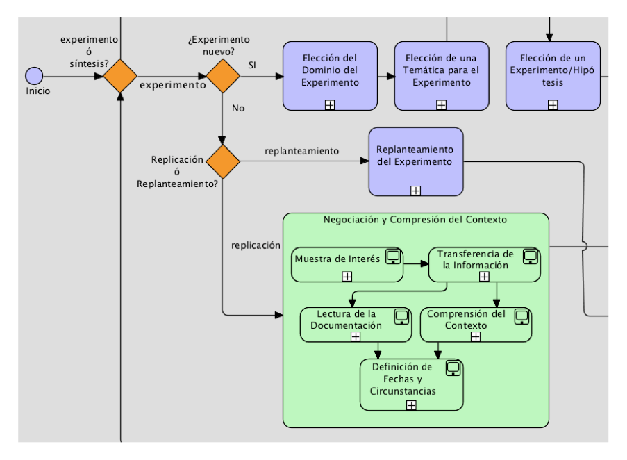
\includegraphics[width=3.2in]{images/Proccess}
	\caption{Diagrama de procesos resultado de las entrevistas semi-estructuradas.}
	\label{fig-proceso-exp}\odnote{RODRIGO: Pon el modelo completo.}\odnote{RODRIGO: No se produjo una evoluci�n de los modelos conceptuales?}
\end{figure}

\begin{figure}[htbp!]
	\centering
	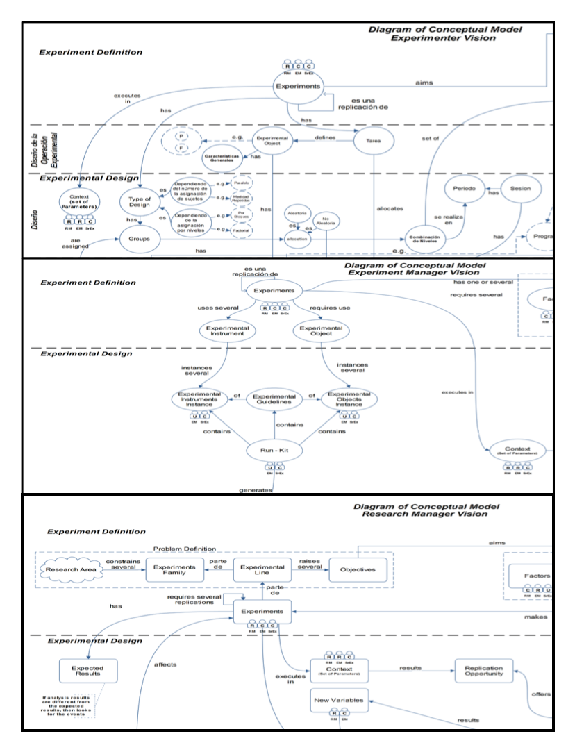
\includegraphics[width=3.4in]{Images/Concepts}
	\caption{Modelos conceptuales finales}\odnote{RODRIGO: Pon el modelo completo. No hay cambios en los modelos de procesos?}
	\label{fig-conceptos-exp}
\end{figure}

\section{Conceptual models of Experimentation on Biotechnology}\label{sec:annex-models-BIO}

\begin{figure}[htbp!]
	\centering
	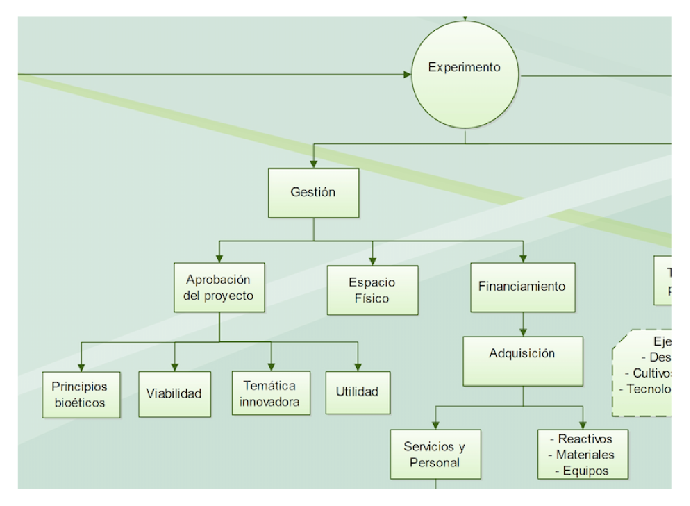
\includegraphics[width=3in]{Images/Concepts-Draft-Bio}
	\caption{Modelo Conceptual Inicial de Biotecnolog�a}
	\label{fig-concepts-initial-bio}\odnote{RODRIGO: Poner modelo completo}.
\end{figure}

\begin{figure}[htbp!]
	\centering
	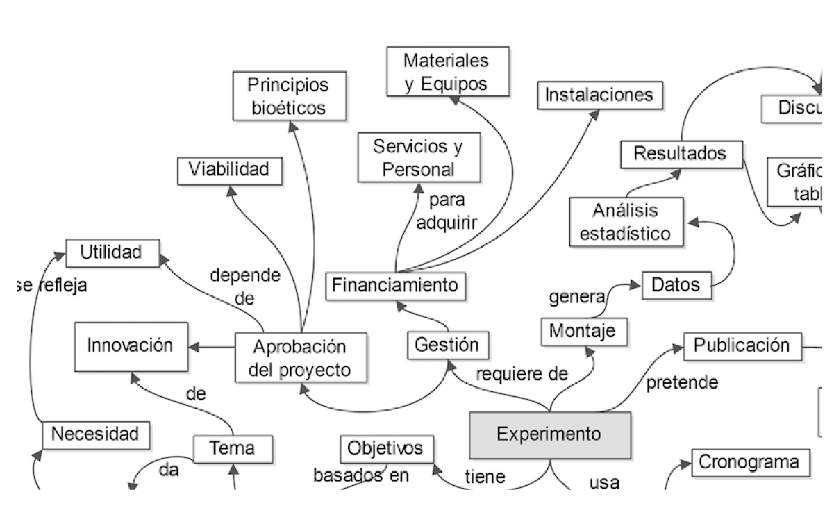
\includegraphics[width=3in]{Images/Concepts-Final-Bio}
	\caption{Modelo Conceptual final de experimentaci�n en Biotecnolog�a}
	\label{fig-concepts-final-bio}\odnote{RODRIGO: Poner modelo completo}.
\end{figure}

\begin{figure}[htbp!]
	\centering
	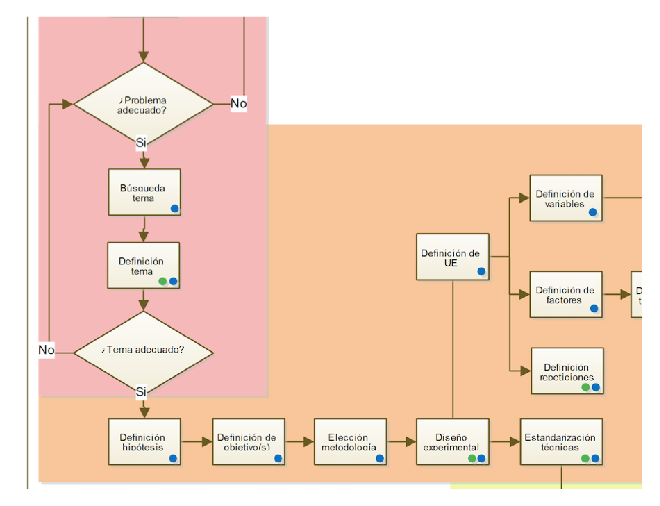
\includegraphics[width=3.2in]{Images/Final-Process}
	\caption{Modelo final del proceso experimental en Biotecnolog�a}
	\label{fig-proceso-exp-final}\odnote{RODRIGO: Poner modelo completo}.
\end{figure}